\section{Параметризация модели движения}
\label{sec:Chapter2} \index{Chapter2}

Параметризованная модель движения представима в следующем виде:

\begin{equation*}
    \ddot{\mathbf{x}} = \mathbf{f}(\mathbf{x}, t) +
    \mathbf{f}_1(a_1, \dots, a_n, t),
\end{equation*}
где к исходной системе уравнений орбитальной динамики добавлена
некоторая функция, зависящая от $n$ параметров.

Неизвестные величины $a_1, \dots, a_n$ должны определяться в ходе процедуры минимизации при
восстановлении орбиты.

В настоящей работе исследуется две параметризации -- псевдоускорения и псевдоимпульсы.

\subsection{Псевдоускорения}

Псевдоускорение -- это дополнительная сила которая действует на КО на некотором участке 
траектории. Как правило, мерный интервал разбивается на несколько участков, и на каждом
из них дополнительная сила постоянна. В некоторых случаях ускорения выбрают не
кусочно-постоянными, а кусочно-линейными для непрерывности производной силы.
Направление ускорений может быть разложено по компонентам орбитальной системы координат на радиальную, тангенциальную и нормальную
составляющие. 

Концептуальная схема применения псевдоускорений изображена на рис. \ref{fig:pseudoacc}.

\begin{figure}[h!]
    \centering
    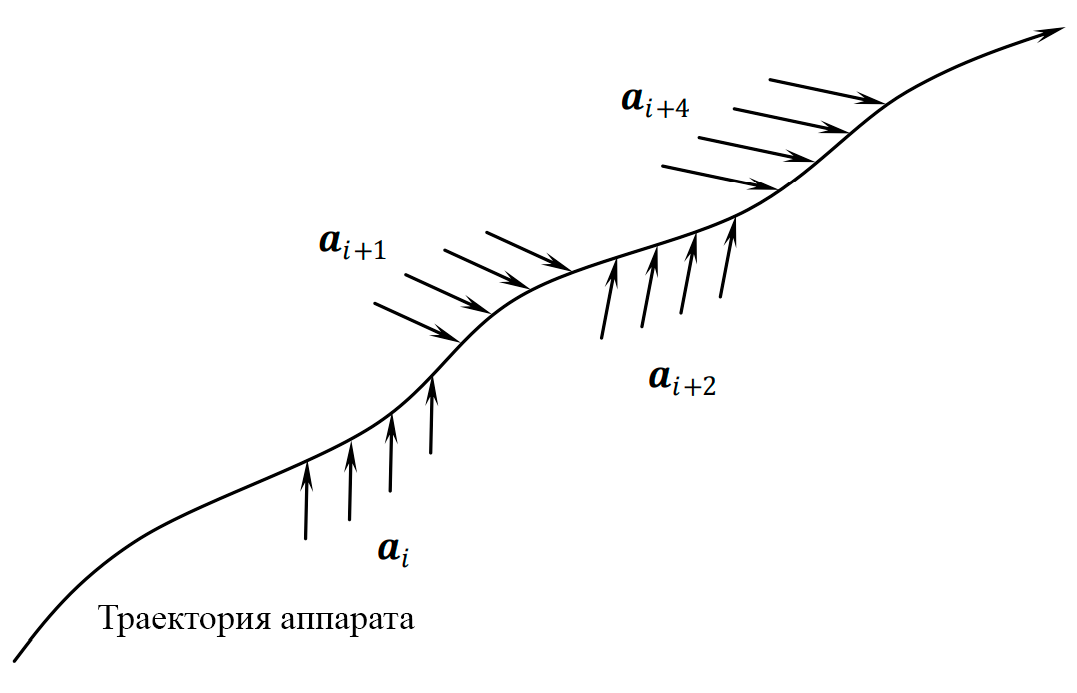
\includegraphics[width=0.8\linewidth]{../images/solution/lageos/pseudoacc.png}
    \captionof{figure}{Схема применения псевдоускорений}
    \label{fig:pseudoacc}
 \end{figure}

Уравнение движение с учетом псевдоимпульсов:
\begin{equation*}
    \ddot{\mathbf{x}} = \mathbf{f}(\mathbf{x}, t) +
        \sum_{i=0}^{n-1} \sum_{j=1}^{3} a_{i,j} \cdot \xi_{i}(t) \cdot \mathbf{e_j} (t),
\end{equation*}
где $a_{i,j}$ -- величина импульса вдоль направления $\mathbf{e_j}$.

\begin{equation*}
    \xi_{i}(t) = 
            \begin{cases}
                0, & t < t_i \\
                1, & t_i < t < t_{i+1} \\
                0, & t_{i+1} \le t
            \end{cases}
\end{equation*}

Столбец матрицы изохронных производных, соответствующий параметру псевдоимпульса,
может быть вычислен в процессе интегрирования уравнения в вариациях аналогично
столбцу производных по площади аэродинамического сопротивления или солнечного давления.

\subsection{Псевдоимпульсы}

Псевдоимпульсы -- мгновенные изменения скорости в определенные моменты времени.
Эти изменения выражаются в разрыве I рода скорости, что приводит к появлению
$\delta$-функции в ускорении. При этом траектория остается непрерывной.

Схематичный вид псевдоимпульсов приведен на рис. \ref{fig:pseudoimp}

\begin{figure}[h!]
    \centering
    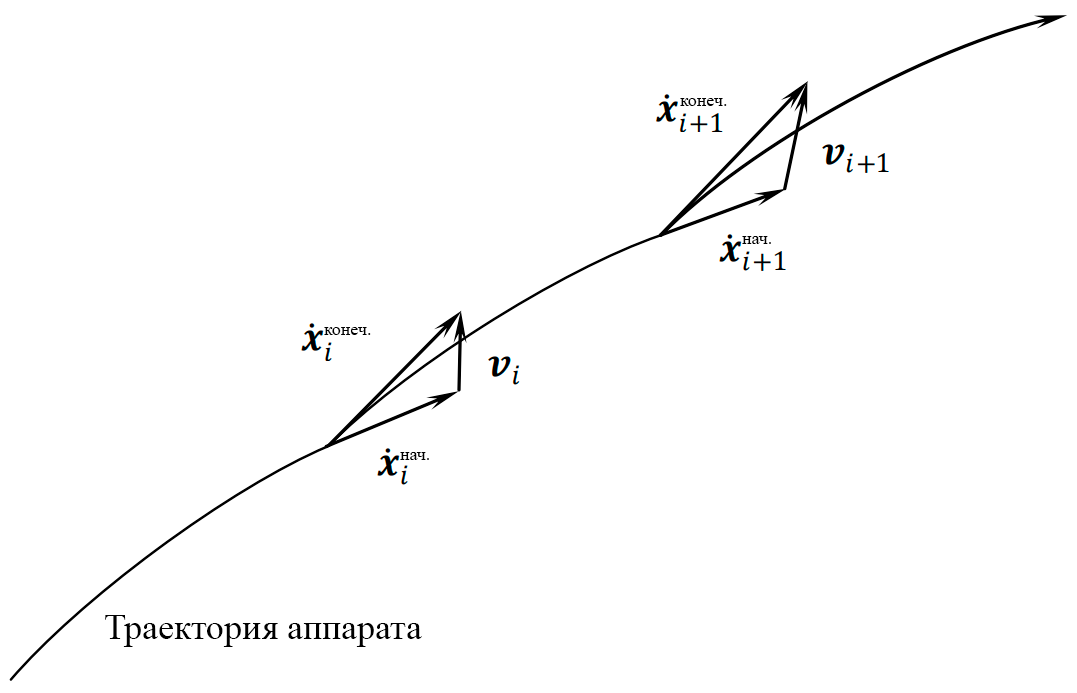
\includegraphics[width=0.8\linewidth]{../images/solution/lageos/pseudoimp.png}
    \captionof{figure}{Схема применения псевдоимпульсов}
    \label{fig:pseudoimp}
 \end{figure}

Динамика движения при наличии псевдоимпульсов описывается выражением:
\begin{equation*}
    \ddot{\mathbf{x}} = \mathbf{f}(\mathbf{x}, t) +
        \sum_{i=0}^{n-1} \sum_{j=1}^{3} v_{i,j} 
                    \cdot \delta (t - t_i) \cdot \mathbf{e_j} (t_i),
\end{equation*}
где $v_{i,j}$ -- величина импульса вдоль направления $\mathbf{e_j}$.

Получим выражение для столбца в матрице изохронных производных, соответствующего одному импульсу.
Введем функцию $U(t)$ как блок размерами 6 на 6 матрицы изохронных производных $\Phi$, отвечающий за
матрицу Якоби мгновенных элементов орбиты $\mathbf{\textbf{Э}}(t)$ по начальным элементам 
$\mathbf{\textbf{Э}}_0$:

\begin{equation*}
    U(t) = \frac{\partial \mathbf{\textbf{Э}}(t)}{\partial \mathbf{\textbf{Э}}_0}
\end{equation*}

Пусть в момент времени $t_0$ был совершен псевдоимпульс.
Представим матрицу Якоби мгновенных элементов орбиты по элементам в момент импульса через $U(t)$:
\begin{equation*}
    \frac{\partial \mathbf{\textbf{Э}}(t)}{\partial \mathbf{\textbf{Э}}(t_0)} = 
    \frac{\partial \mathbf{\textbf{Э}}(t)}{\partial \mathbf{\textbf{Э}}_0} \cdot
    \frac{\partial \mathbf{\textbf{Э}}_0}{\partial \mathbf{\textbf{Э}}(t_0)} = 
    U(t) \cdot U(t_0)^{-1}
\end{equation*}

Используя полученные уравнения, можно получить искомый столбец при $t > t_0$:
\begin{equation*}
    \frac{\partial \mathbf{\textbf{Э}}(t)}{\partial \mathbf{\textbf{Э}}(t_0)} = 
    \frac{\partial \mathbf{\textbf{Э}}(t)}{\partial \mathbf{\textbf{Э}}(t_0)} \cdot
    \frac{\partial \mathbf{\textbf{Э}(t_0)}}{\partial \mathbf{v}_{t_0}} =
    U(t) \cdot U(t_0)^{-1} \cdot
    \frac{\partial \mathbf{\textbf{Э}(t_0)}}{\partial \mathbf{v}_{t_0}}
\end{equation*}

При $t < t_0$ данный столбец равен соответствующему столбцу единичной матрицы, 
так как импульс еще не был соверешен.

Заметим, что рассмотренные столбцы могут быть вычислены с минимальными дополнительными
ресурсами, так как используется уже имеющееся после прогноза решение уравения в вариациях.

\subsection{Верификация}

Тестирование программного комплекса проводилась на КА LAGEOS-2.
Измерения орбиты данного аппарата выполняются с помощью лазерной дальнометрии.
Высокоточные эфемериды LAGEOS-2 публикуются рядом агентств, 
в том числе итальянским и немецким исследовательскими центрами. Эти орбиты
были выбраны в качестве референсных. 

Сравнение эфемерид агентств показано на рисунке \ref{fig:compare_agencies}. Средняя
норма разницы по положению составляет 3 сантиметра, а стандартное отклонение -- 2 сантиметра. 
Пики на графике -- псевдоимпульсы, применяемые итальянским агентством. В дальнейшем Сравнение
будет проводиться именно с ним.

\begin{figure}[h!]
    \centering
    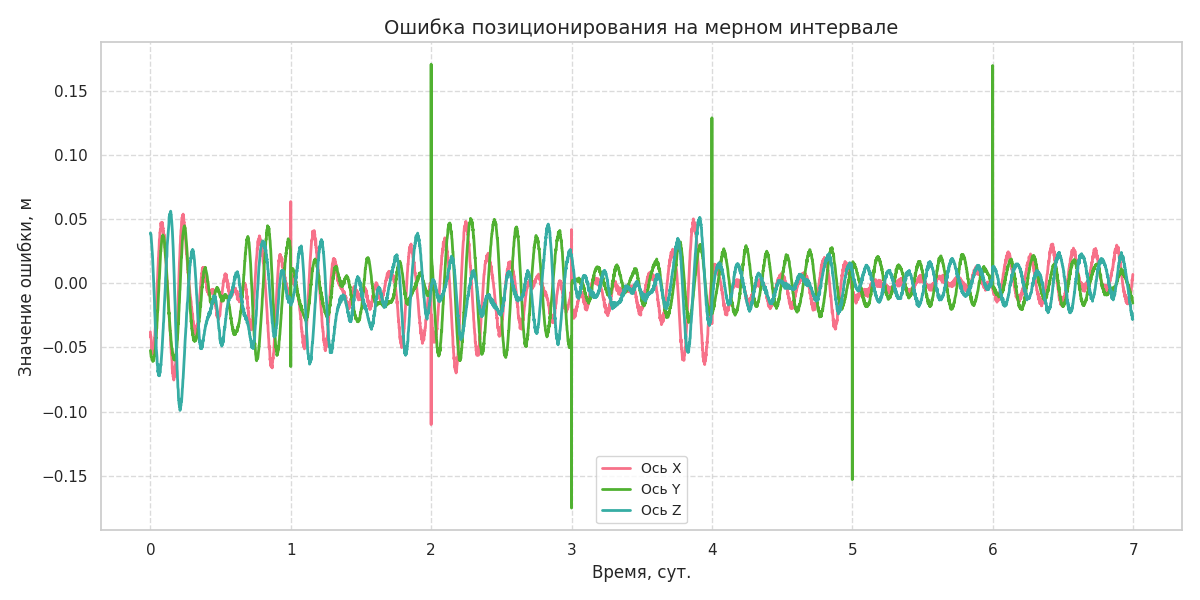
\includegraphics[width=\linewidth]{../images/solution/lageos/compare_agencies.png}
    \captionof{figure}{Разница между итальнским и немцким агентствами на мерном интервале}
    \label{fig:compare_agencies}
 \end{figure}

Характеристики аппарата и общие сведения об орбите отражены в таблицах \ref{tab:lageos2}
и \ref{tab:lageos2_orb}.

\begin{table}[h!]
    \centering
    \begin{minipage}[t]{0.48\textwidth}
    \centering
    \renewcommand{\arraystretch}{1.5}
    \begin{tabular}{|l|l|}
    \hline
    \multicolumn{2}{|c|}{Параметры аппарата} \\ \hline
    Форма       & Сфера      \\ \hline
    Диаметр     & 60 см      \\ \hline
    Вес         & 405.38 кг  \\ \hline
    \end{tabular}
    \caption{Параметры аппарата LAGEOS-2}
    \label{tab:lageos2}
    \end{minipage}
    \hfill
    \begin{minipage}[t]{0.48\textwidth}
    \centering
    \renewcommand{\arraystretch}{1.5}
    \begin{tabular}{|l|l|}
    \hline
    \multicolumn{2}{|c|}{Параметры орбиты} \\ \hline
    Перигей        & 5620 км   \\ \hline
    Наклонение     & 52.64°    \\ \hline
    Эксцентриситет & 0.0135    \\ \hline
    Период         & 223 мин.  \\ \hline
    \end{tabular}
    \caption{Параметры орбиты LAGEOS-2}
    \label{tab:lageos2_orb}
    \end{minipage}
\end{table}

Для тестирования была реализована модель движения близкая к модели агентства.
Ключевые характеристики модели представлены в таблице \ref{tab:lageos2_forces}.
Помимо геопотенциала с приливными поправками учитывалось притяжение третьих тел,
солнечное давление, эффект альбедо и релятивистские поправки. Также были применены
рассмотренные выше псевдоускорения и псевдоимпульсы. 

\begin{table}[h!]
    \centering
    \renewcommand{\arraystretch}{1.5}
    \begin{tabular}{|ll|}
    \cline{1-2}
    \multicolumn{2}{|c|}{Параметры модели движения}                                                                                                                                                 \\ \hline
    \multicolumn{1}{|l|}{Геопотенциал}           & \begin{tabular}[l]{@{}l@{}}GGM02C, 70 гармоник.\\ Твердотельные и океанические \\поправки по IERS\end{tabular}                      \\ \hline
    \multicolumn{1}{|l|}{Притяжение третьих тел} & \begin{tabular}[l]{@{}l@{}}Планеты: Солнце, Меркурий, Венера, Луна, \\ Марс, Юпитер, Сатурн, Уран, Нептун.\\ Эфемериды:  JPL DE403\end{tabular} \\ \hline
    \multicolumn{1}{|l|}{Солнечное давление}     & Модель тени с перекрытием                                                                                                               \\ \hline
    \multicolumn{1}{|l|}{Эффект альбедо}         & Модель Кноке                                                                                                                            \\ \hline
    \multicolumn{1}{|l|}{Эмпирика}               & \begin{tabular}[l]{@{}l@{}}7 псевдоускорений,\\ 7 псевдоимпульсов.\\ Равномерно распределены \\ на мерном интервале\end{tabular}        \\ \hline
    \multicolumn{1}{|l|}{Релятивистские эффекты}         & по IERS                                                                                                                         \\ \hline
    \end{tabular}
    \caption{Параметры модели движения LAGEOS-2}
    \label{tab:lageos2_forces}
\end{table}

Прогноз траектории выполнялся
методом Эверхарта 15 порядка, длина шага составила 400 секунд. 
Уточненине орбиты проводилось на мерном интервале длиной 7 суток методом Гаусса-Ньютона. 
Параметры уточнения орбиты отражены в таблице \ref{tab:lageos2_opt}.

\begin{table}[h!]
    \centering
    \renewcommand{\arraystretch}{1.5}
    \begin{tabular}{|ll|}
    \hline
    \multicolumn{2}{|c|}{Параметры уточнения орбиты}                                                                                \\ \hline
    \multicolumn{1}{|l|}{Интегрирование}  & \begin{tabular}[c]{@{}l@{}}Метод Эверхарта 15 порядка\\ с шагом 400 секунд\end{tabular} \\ \hline
    \multicolumn{1}{|l|}{Оптимизация}     & Метод Гаусса-Ньютона                                                                    \\ \hline
    \multicolumn{1}{|l|}{Тип измерений}   & Положение, скорость                                                                     \\ \hline
    \multicolumn{1}{|l|}{Целевая функция} & Сумма квадратов невязок                                                                 \\ \hline
    \multicolumn{1}{|l|}{Мерный интервал} & 7 суток (30.05.2021 -- 06.06.2021)                                                                                 \\ \hline
    \end{tabular}
    \caption{Параметры уточнения орбиты}
    \label{tab:lageos2_opt}
\end{table}

Проведена серия численных экспериментов, в которых модель сил поэтапно дополнялась.
Это позволило увидеть динамику снижения ошибки на мерном интервале при учете различных
факторов. Результаты экспериментов представлены в таблице \ref{tab:lageos2_exp}. 

\begin{table}[h!]
    \centering
    \renewcommand{\arraystretch}{1.5}
    \begin{tabular}{|l|lll|}
    \hline
    \multicolumn{1}{|c|}{\multirow{2}{*}{Набор сил}} & \multicolumn{3}{c|}{Ошибка на мерном интервале, м}                                                             \\ \cline{2-4} 
    \multicolumn{1}{|c|}{}                           & \multicolumn{1}{c|}{Максимальная} & \multicolumn{1}{c|}{Средняя} & \multicolumn{1}{c|}{Стандартное отклонение} \\ \hline
    Потенциал с J2                                   & \multicolumn{1}{l|}{432}          & \multicolumn{1}{l|}{161}     & 183                                         \\ \hline
    70 гармоник                                      & \multicolumn{1}{l|}{327}          & \multicolumn{1}{l|}{96}      & 115                                         \\ \hline
    + притяжение третьих тел                         & \multicolumn{1}{l|}{7.4}          & \multicolumn{1}{l|}{2.3}     & 2.7                                         \\ \hline
    + солнечное давление                             & \multicolumn{1}{l|}{2.8}          & \multicolumn{1}{l|}{0.9}     & 1.0                                         \\ \hline
    + приливные поправки                             & \multicolumn{1}{l|}{0.76}         & \multicolumn{1}{l|}{0.26}    & 0.29                                        \\ \hline
    + эффект альбедо                                 & \multicolumn{1}{l|}{0.48}         & \multicolumn{1}{l|}{0.13}    & 0.15                                        \\ \hline
    + 7 псевдоускорений                              & \multicolumn{1}{l|}{0.29}         & \multicolumn{1}{l|}{0.10}    & 0.11                                        \\ \hline
    + 7 псевдоимпульсов                              & \multicolumn{1}{l|}{0.26}         & \multicolumn{1}{l|}{0.05}    & 0.06                                        \\ \hline
    \end{tabular}
    \caption{Зависимость точности восстановления орбиты от учета различных наборов
    возмущающих факторов}
    \label{tab:lageos2_exp}
\end{table}

Из результатов следует, что основные возмущающие факторы -- это нецентральность поля Земли,
притяжение третьих тел и солнечное давление. Учет этих сил позволяет получить среднюю
ошибку на мерном интервале меньше метра. Вклад приливных поправок и эффекта альбедо
значительно меньше. Таким образом, полная модель сил без параметризации дает среднюю ошибку
13 см.

Получить дециметровую точность помогает использвоние псевдоускорений. Данный подход
существенно уменьшает максимальную ошибку и сводит среднюю невзяку и стандартное отклонение
 к 10 и 11 сантиметрам соответственно. Для восстановления орбиты с субдециметровой точностью
 можно повышать количество псевдоускорений или добавить псевдоимпульсы. С комбинацией
 из 7 ускорений и 7 псевдоимпульсов средняя ошибка на мерном интервале падает до 5 см. 
 Такое значение ошибок близко к разнице между двумя агентствами, поэтому
 уточнение орбиты можно считать успешным.

Графики невязок на мерном интервале показаны на рисунках \ref{fig:no_imp_no_acc}, 
\ref{fig:no_imp_with_acc}, \ref{fig:with_imp_with_acc}.

\begin{figure}[h!]
   \centering
   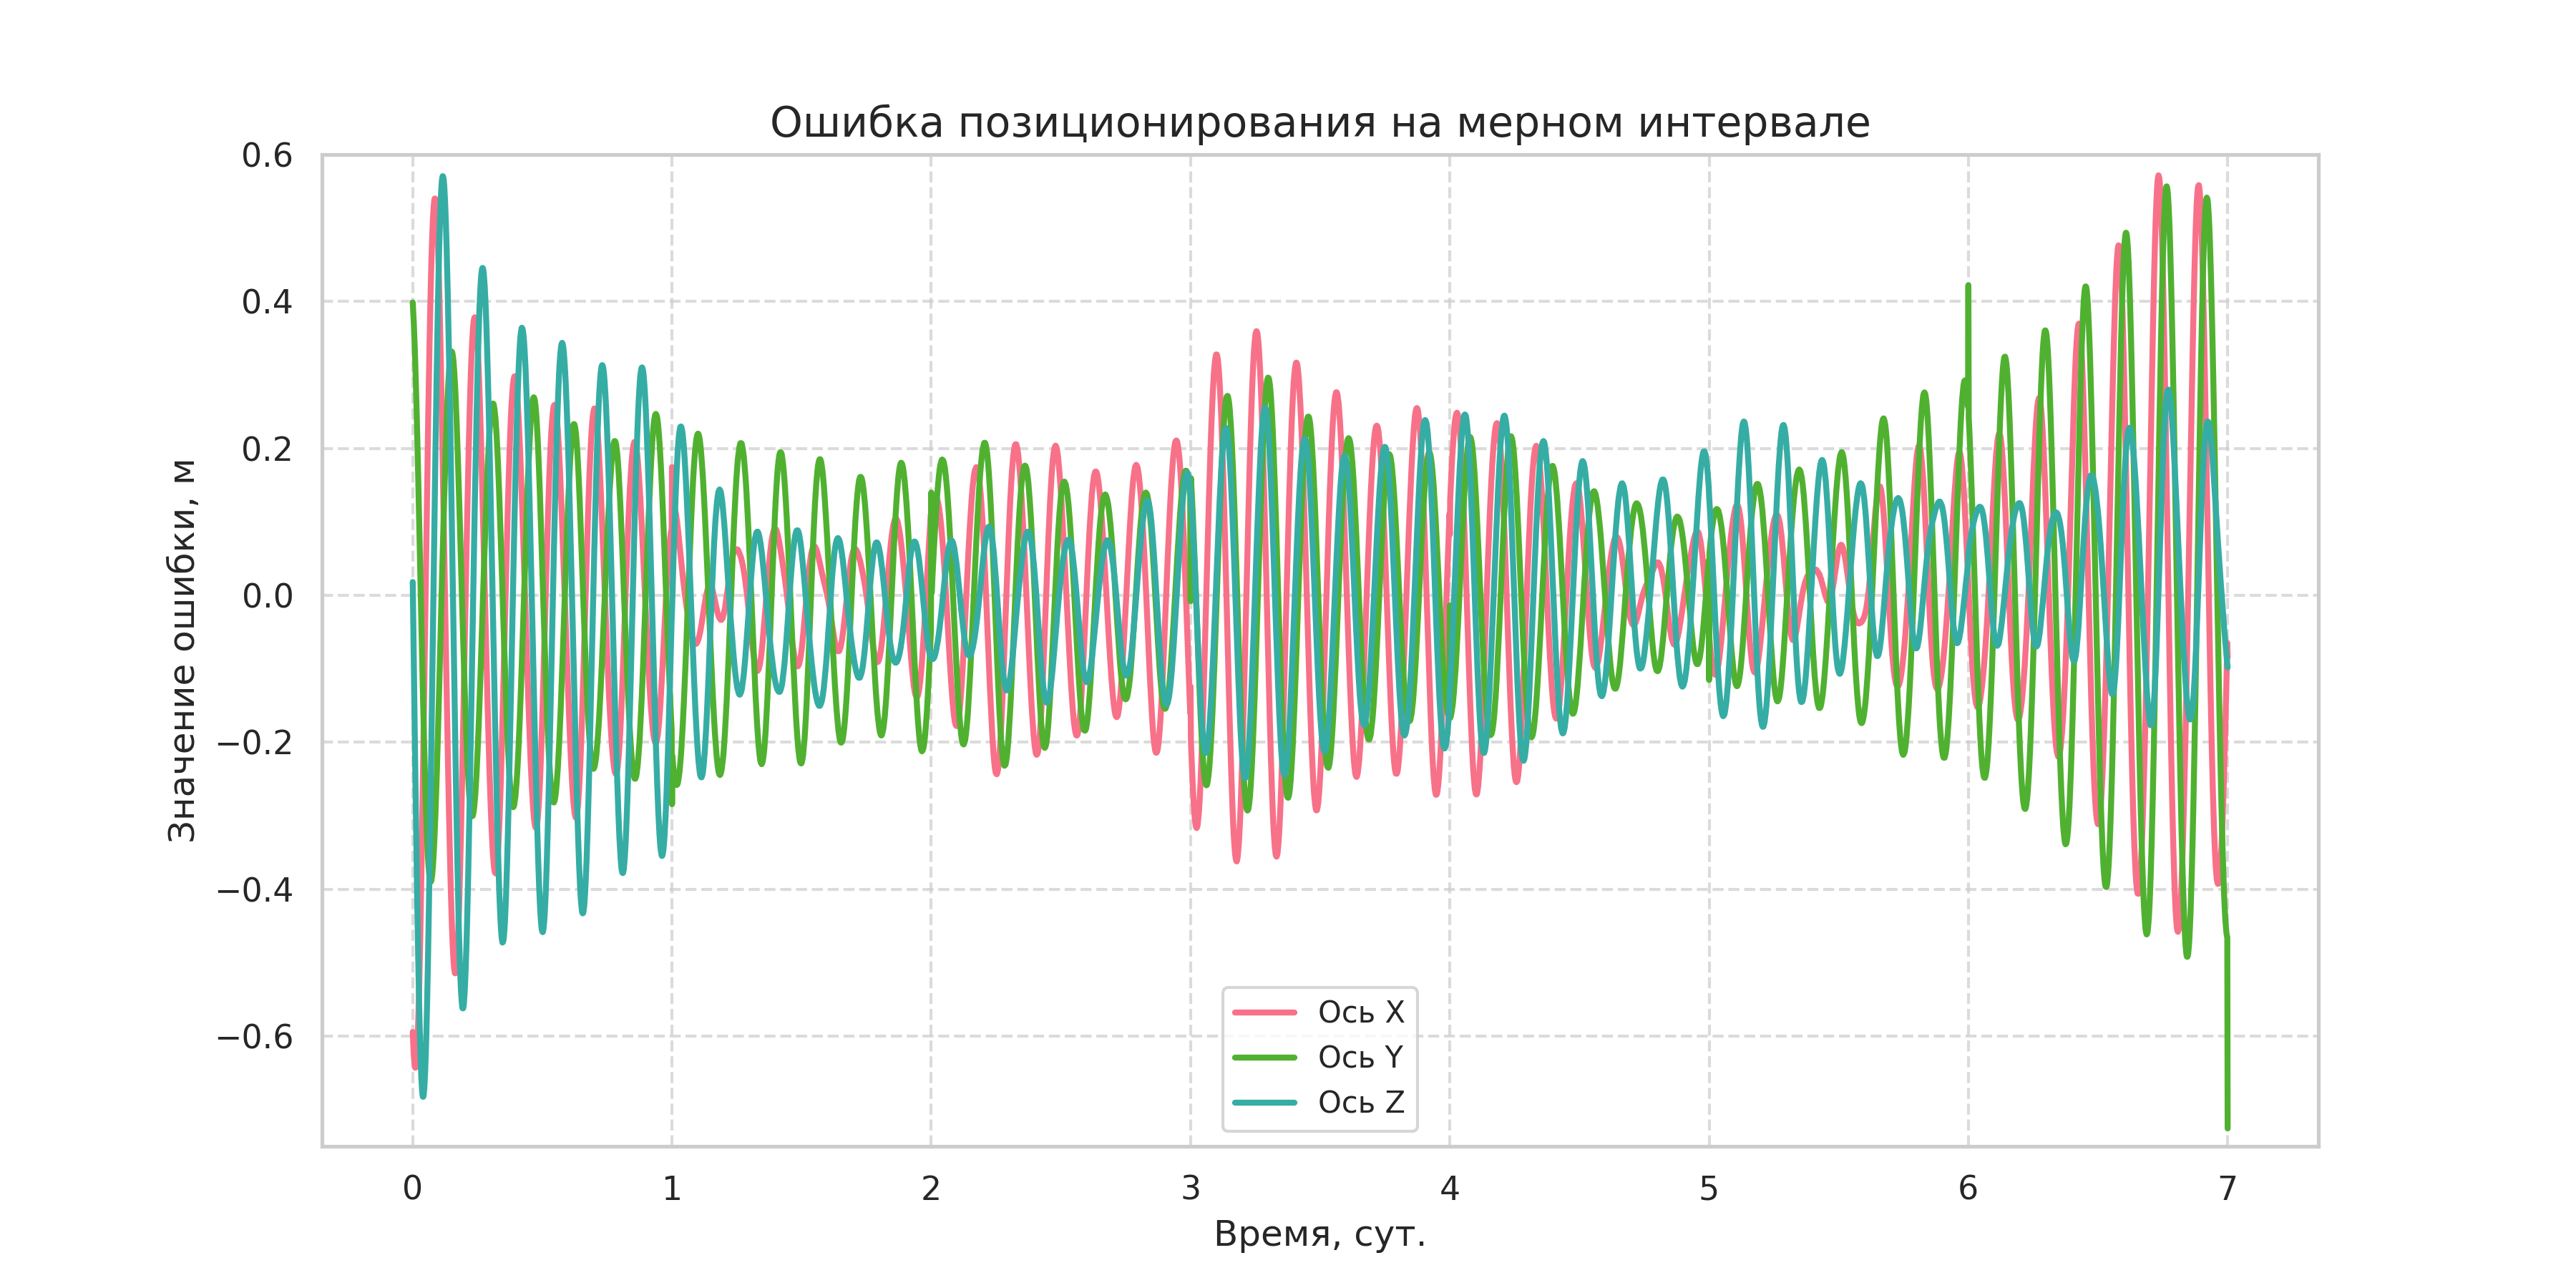
\includegraphics[width=\linewidth]{../images/solution/lageos/no_imp_no_acc.png}
   \captionof{figure}{График невязок на мерном интервале при использовании модели сил без параметризации}
   \label{fig:no_imp_no_acc}
\end{figure}

\begin{figure}[h!]
   \centering
   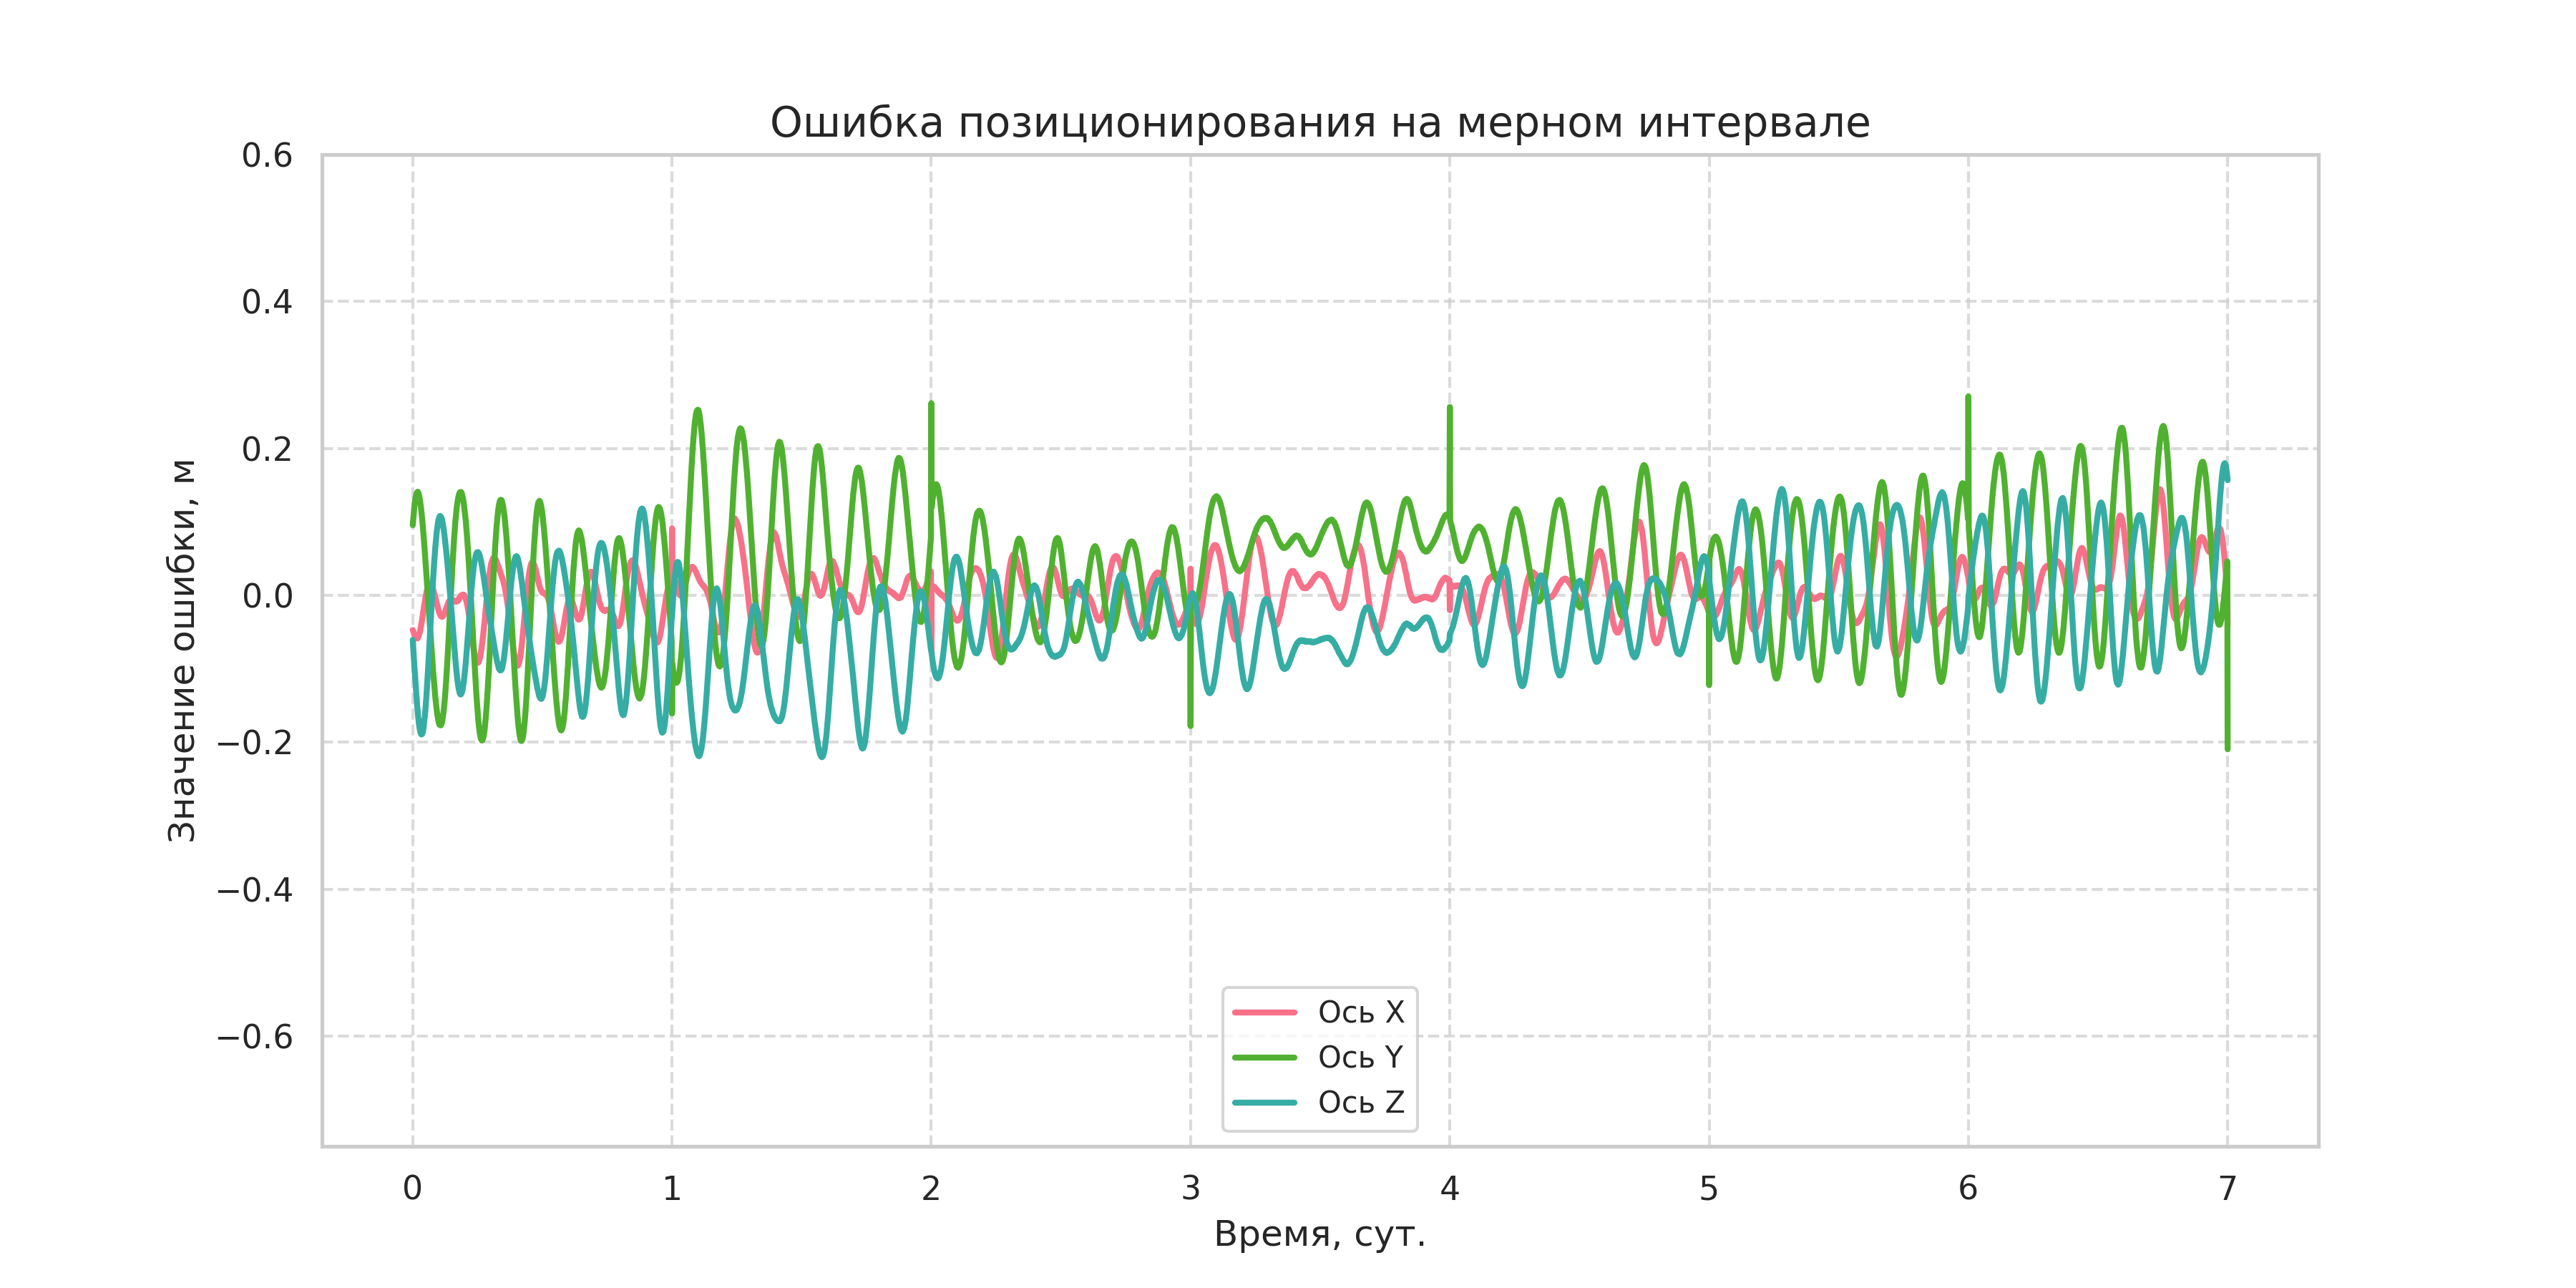
\includegraphics[width=\linewidth]{../images/solution/lageos/no_imp_with_acc.png}
   \captionof{figure}{График невязок на мерном интервале при использовании модели сил c псевдоускорениями}
   \label{fig:no_imp_with_acc}
\end{figure}

\begin{figure}[h!]
   \centering
   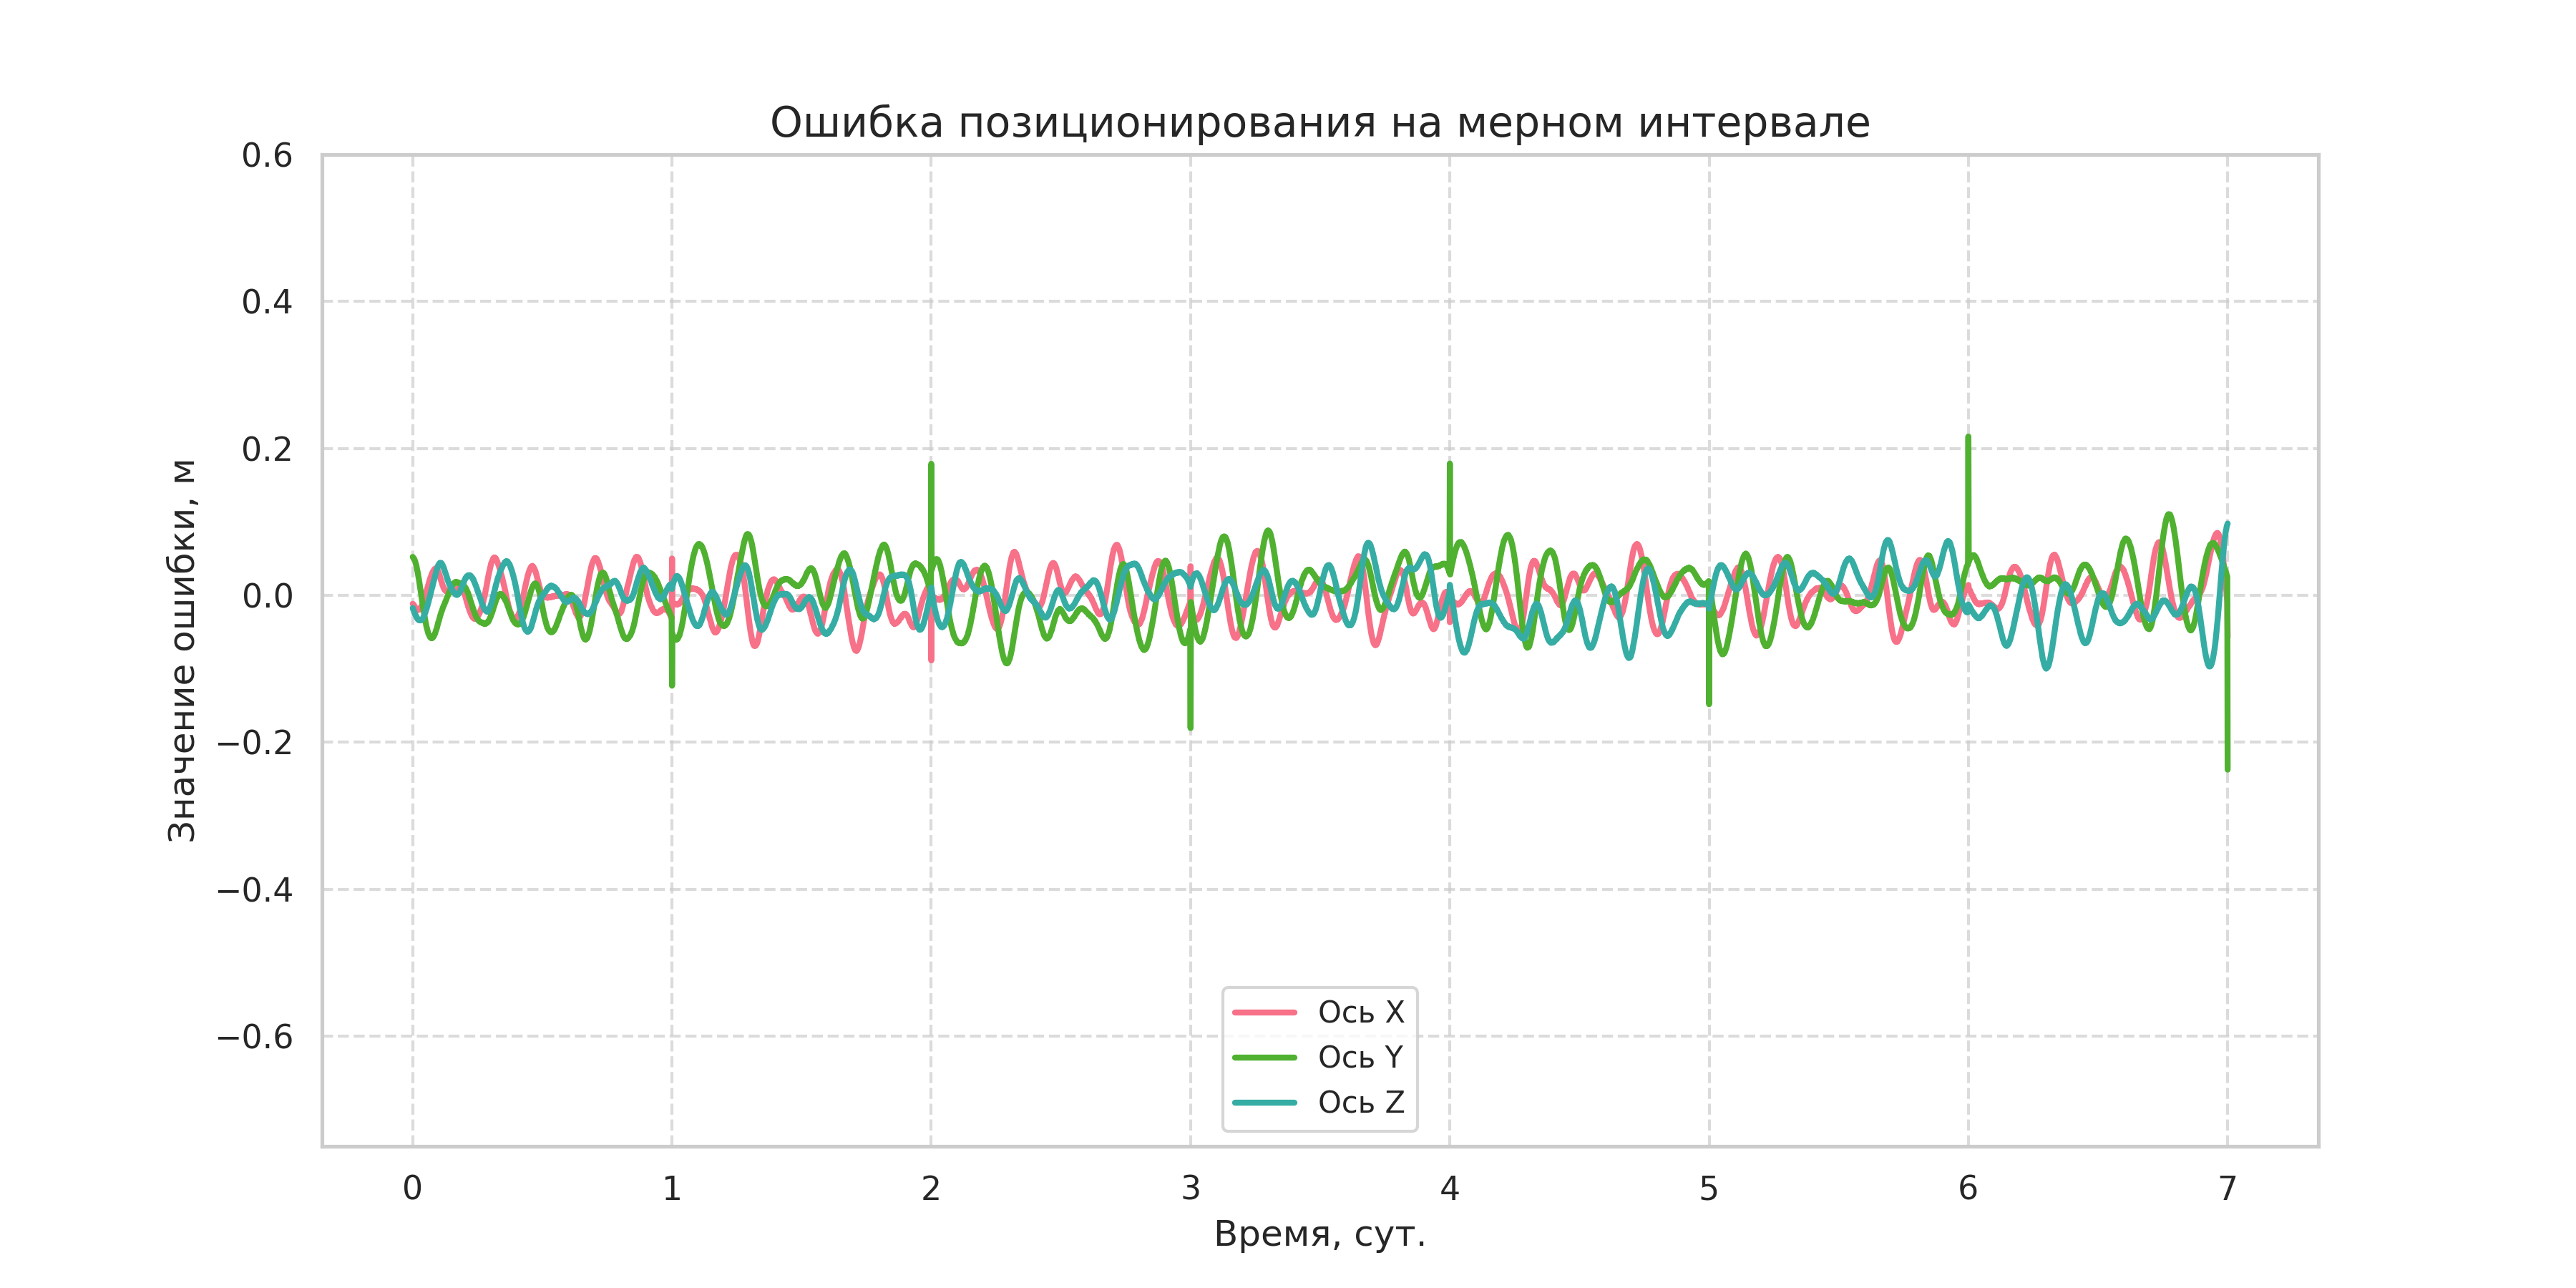
\includegraphics[width=\linewidth]{../images/solution/lageos/with_imp_with_acc.png}
   \captionof{figure}{График невязок на мерном интервале при использовании модели сил с псевдоускорениями
   и псевдоимпульсами}
   \label{fig:with_imp_with_acc}
\end{figure}

На рисунке \ref{fig:no_imp_no_acc} хорошо видна специфика работы метода наименьших квадратов.
Метод оптимизрует решение таким образом, что в центральной области невязка получается
минимальной, а по краям симметрично растет. Это свидетельствует о правильной работе
алгоритма восстановления орбиты.

Верификация пройдена.